\chapter{Failures of the Relativistic Quantum Mechanics}

In this chapter we will discuss the problems of relativistic quantum mechanics. We will start
with the problem of probability density. We will show that the probability density is positive-definite for Dirac Equation
but is not in the case of the Klein-Gordon equation. Then we will TODO:

\section{Probability density}

\paragraph{} In the non-relativistic case we can find the continuity equation by taking the complex conjugate
of the Schrodinger's equation.

\begin{equation*}
    \begin{gathered}
        i \hbar \partialder{}{t} \psi = \hat{H} \psi \\
        - i \hbar \partialder{}{t} \psi^{*} = \big(\hat{H} \psi \big)^{*}
    \end{gathered}
\end{equation*}

Then we mutiply the first equation by $\psi$ and the second one by $\psi^{*}$.

\begin{equation*}
    \begin{gathered}
        i \hbar \psi^{*} \partialder{}{t} \psi = \psi^{*} \hat{H} \psi \\
        i \hbar \psi \partialder{}{t} \psi^{*} = \psi \big(\hat{H} \psi \big)^{*}
    \end{gathered}
\end{equation*}

If we substract these two equations from each other and use the formula for derivative $(a \cdot b)' = a' \cdot b + a \cdot b'$
we wil get a form from which it will be easy to identify the continuity equation $\partialder{\rho}{t} + div \vec{j} = 0$.

\begin{equation*}
    i \hbar \partialder{\left|\psi\right|^{2}}{t}  = \psi^{*} \hat{H} \psi - \psi \big(\hat{H} \psi \big)^{*}
\end{equation*}

We assume the potential $V$ in $\hat{H} = \frac{\hat{p}^{2}}{2m} + V$ to be real-valued thus the right-hand side
will simplify to

\begin{equation*}
    \psi^{*} \frac{\hbar^{2}}{2m} \nabla^{2} \psi - \psi \frac{\hbar^{2}}{2m} \nabla^{2} \psi^{*} 
    = \frac{\hbar^{2}}{2m} \bigg( \psi^{*} \nabla^{2} \psi - \psi \nabla^{2} \psi^{*} \bigg)
\end{equation*}

and the desired form is

\begin{equation*}
    \partialder{\left|\psi\right|^{2}}{t} + div \bigg[ \frac{\hbar}{2mi} \bigg( \psi \nabla \psi^{*} - \psi^{*} \nabla \psi \bigg) \bigg] = 0
\end{equation*}

Now we will do the same for the Klein-Gordon equation \ref{eq:klein_gordon}. Let's do the same procedure here and
find the complex conjugate, multiply both equations by $\psi$ and $\psi^{*}$ and then substract them. After that 
let's focus on the term which contains the time derivative a thus will represent the \textit{probability density}.

\begin{equation*}
    \partialder{\rho}{t} \sim \frac{1}{2i} \bigg[ \psi^{*} \partialdernd{}{t} \psi - \psi \partialdernd{}{t} \psi^{*} \bigg]
\end{equation*}

Now we can find what $\rho$ is proportial to. 

\begin{equation}
    \rho \sim \frac{1}{2i} \bigg[ \psi^{*} \partialder{}{t} \psi - \psi \partialder{}{t} \psi^{*} \bigg]
\end{equation}

Let's divide the wave function $\psi$ into the real and imaginary part.

\begin{equation*}
    \begin{gathered}
        \psi = i \psi_{1} + \psi_{2} \\
        \rho \sim \bigg[ \psi_{2} \partialder{}{t} \psi_{1} - \psi_{1} \partialder{}{t} \psi_{2} \bigg]
    \end{gathered}
\end{equation*}

Now it is easy to see the problem. In the non-relativistic case the probability density was simply $|\psi|^{2}$ which is
non-negative for any $\psi: \mathbb{R} \to \mathbb{C}$. In the case of Klein-Gordon equation, we can see the probability 
density is zero whenever the wave function is either exclusively real or imaginary. Moreover, since both 
$\partialder{\psi_{1}}{t}$ and $\partialder{\psi_{2}}{t}$ are arbitrary, the value can be negative. This is in contradiction
with the intepretation of $\rho$ as the \textit{probability density of measuring the system within a given state $\psi$}.
To solve this problem, Dirac introduced his equation. Let's check the probability density using the procedure of deriving
the continuity equation from the Dirac equation \cite{dirac_equation_history}. Let's start with the Dirac equation of the 
form as follows.

\begin{equation}
    \label{eq:dirac_equation}
    (i \hbar \gamma^{\mu} \partial_{\mu} - mc) \psi = 0
\end{equation}

For further discussion let's introduce some useful theorems.

\begin{theorem}
    \label{th:gamma_matrices}
    Let $\gamma^{\mu}$'s be Dirac matrices \cite{gamma_matrices} defined by the properties (see \cite{dirac_matrices})

    \begin{equation}
        \label{eq:gamma_matrices_def_1}
        \begin{gathered}
            \big\{\gamma^{\mu}, \gamma^{\nu}\big\} = 2 \eta^{\mu \nu} I_{4}
        \end{gathered}
    \end{equation}

    where $\eta^{\mu \nu} = diag\{+1, -1, -1, -1\}$, and

    \begin{equation}
        \label{eq:gamma_matrices_def_2}
        \begin{gathered}
            \big(\gamma^{\mu}\big)^{\dagger} = \gamma^{0} \gamma^{\mu} \gamma^{0}
        \end{gathered}
    \end{equation}

    then following equations hold for $\mu \in \{0, 1, 2, 3\}$, $i \in \{1, 2, 3\}$.

    \begin{equation}
        \label{eq:gamma_matrices_1}
        \gamma^{0} \gamma^{i} = - \gamma^{i} \gamma^{0}
    \end{equation}

    \begin{equation}
        \label{eq:gamma_matrices_2}
        \begin{gathered}
            \big(\gamma^{0}\big)^{\dagger} = \gamma^{0} \\
            \big(\gamma^{i}\big)^{\dagger} = - \gamma^{i}
        \end{gathered}
    \end{equation}

\end{theorem}

\begin{proof}
    The proof of \ref{eq:gamma_matrices_1} is a direct application of the definition \ref{eq:gamma_matrices_def_1}.

    \begin{equation*}
        \begin{gathered}
            \{\gamma^{0}, \gamma^{i}\} = \gamma^{0} \gamma^{i} + \gamma^{0} \gamma^{i} = 2 \eta^{0 i} I_{4} \\
            \gamma^{0} \gamma^{i} + \gamma^{0} \gamma^{i} = 0 \\
            \gamma^{0} \gamma^{i} = - \gamma^{0} \gamma^{i} 
        \end{gathered}
    \end{equation*}

    To proof \ref{eq:gamma_matrices_2} we just need to know that $\gamma^{0} \gamma^{0} = I_{4}$ which can be shown to be true because we
    constructed the matrices to be so or by checking the definition \ref{eq:gamma_matrices_def_1}: 
    $\{\gamma^{0}, \gamma^{0}\} = 2 \gamma^{0} \gamma^{0} = 2 \eta^{00} I_{4}$. Then we use the defining property 
    \ref{eq:gamma_matrices_def_2} and the equation \ref{eq:gamma_matrices_1}.

    \begin{equation*}
        \begin{gathered}
            \big(\gamma^{0}\big)^{\dagger} = \gamma^{0} \gamma^{0} \gamma^{0} = \gamma^{0} I_{4} = \gamma^{0} \\
            \big(\gamma^{i}\big)^{\dagger} = \gamma^{0} \gamma^{i} \gamma^{0} = - \gamma^{0} \gamma^{0} \gamma^{i} = - I_{4} \gamma^{i} = - \gamma^{i}
        \end{gathered}
    \end{equation*}

\end{proof}

We will use a similar trick we used within the Schrodinger equation or the Klein-Gordon equation. We
take the Hermitian adjoint of the left-hand side of the Dirac equation \ref{eq:dirac_equation}.

\begin{equation*}
    \begin{gathered}
        \big[i \hbar \gamma^{\mu} \partial_{\mu} \psi - mc \psi\big]^{\dagger} = \\
        = \big[i \hbar \gamma^{0} \partial_{0} \psi + \gamma^{1} \partial_{1} \psi + \gamma^{2} \partial_{2} \psi + \gamma^{3} \partial_{3} \psi - mc \psi\big]^{\dagger} = \\
        = - i \hbar \big[\big(\gamma^{0} \partial_{0} \psi\big)^{\dagger} + \big(\gamma^{1} \partial_{1} \psi\big)^{\dagger} + 
            \big(\gamma^{2} \partial_{2} \psi\big)^{\dagger} + \big(\gamma^{3} \partial_{3} \psi \big)^{\dagger}\big] - mc \psi^{\dagger} = \\
        = - i \hbar \big[ \partial_{0} \psi^{\dagger} (\gamma^{0})^{\dagger} + \partial_{1} \psi^{\dagger} (\gamma^{1})^{\dagger} + \partial_{2} \psi^{\dagger} (\gamma^{2})^{\dagger}
            + \partial_{3} \psi^{\dagger} (\gamma^{3})^{\dagger} \big] - mc \psi^{\dagger}
    \end{gathered}
\end{equation*}

By using the equation \ref{eq:gamma_matrices_2} we evaluate all the gamma matrices with a dagger.

\begin{equation}
    \label{eq:conjugate_dirac_equation}
    - i \hbar \big[ \partial_{0} \psi^{\dagger} \gamma^{0} + \partial_{1} \psi^{\dagger} (- \gamma^{1}) + \partial_{2} \psi^{\dagger} (-\gamma^{2})
        + \partial_{3} \psi^{\dagger} (-\gamma^{3}) \big] - mc \psi^{\dagger} = 0
\end{equation}

Now, the trick is to introduce $\overline{\psi} := \psi^{\dagger} \gamma^{0}$, multiply the equation \ref{eq:conjugate_dirac_equation} by 
$\gamma^{0}$ from the right and then rewrite all the $\psi^{\dagger} \gamma^{0}$ terms with $\overline{\psi}$ using the equation \ref{eq:gamma_matrices_1}.

\begin{equation*}
    \begin{gathered}
        - i \hbar \big[ \partial_{0} \psi^{\dagger} \gamma^{0} \gamma^{0} + \partial_{1} \psi^{\dagger} (- \gamma^{1} \gamma^{0}) + \partial_{2} \psi^{\dagger} (-\gamma^{2} \gamma^{0})
            + \partial_{3} \psi^{\dagger} (-\gamma^{3} \gamma^{0}) \big] - mc \psi^{\dagger} \gamma^{0} = 0 \\
        - i \hbar \big[ \partial_{0} \psi^{\dagger} \gamma^{0} \gamma^{0} + \partial_{1} \psi^{\dagger} (\gamma^{0} \gamma^{1}) + \partial_{2} \psi^{\dagger} (\gamma^{0} \gamma^{2})
            + \partial_{3} \psi^{\dagger} (\gamma^{0} \gamma^{2}) \big] - mc \psi^{\dagger} \gamma^{0} = 0 \\
        - i \hbar \big[ \partial_{0} \overline{\psi} \gamma^{0} + \partial_{1} \overline{\psi} \gamma^{1} + \partial_{2} \overline{\psi} \gamma^{2}
            + \partial_{3} \overline{\psi} \gamma^{2} \big] - mc \overline{\psi} = 0 \\
    \end{gathered}
\end{equation*}

And finally, we will multiply this equation by $\psi$ from the left.

\begin{equation}
    i \hbar \partial_{\mu} \overline{\psi} \gamma^{\mu} \psi + mc \overline{\psi} \psi = 0
\end{equation}

To get rid of the $mc \overline{\psi} \psi$ term, let's take the original equation \ref{eq:dirac_equation} and multiply it
by $\overline{\psi}$ from the right. Then we will simply add these two equations

\begin{equation*}
    \begin{gathered}
        i \hbar \partial_{\mu} \overline{\psi} \gamma^{\mu} \psi + mc \overline{\psi} \psi = 0 \, \land \,
        i \hbar \overline{\psi} \gamma^{\mu} \partial_{\mu} \psi - mc \overline{\psi} \psi = 0 \implies \\
        \partial_{\mu} \overline{\psi} \gamma^{\mu} \psi + \overline{\psi} \gamma^{\mu} \partial_{\mu} \psi = 0
    \end{gathered}
\end{equation*}

\begin{equation}
    \label{eq:dirac_continuity}
    \partial_{\mu} (\overline{\psi} \gamma^{\mu} \psi) = 0
\end{equation}

From the continuity equation \ref{eq:dirac_continuity} we see that the probability density should be $\rho = \overline{\psi} \gamma^{0} \psi$.
Which is

\begin{equation*}
    \rho = \overline{\psi} \gamma^{0} \psi = \psi^{\dagger} \gamma^{0} \gamma^{0} \psi = \psi^{\dagger} \psi
\end{equation*}

and thus always a positive quantity! TODO: discussion on the results.

\section{Ground state}

\section{Causality}

Now we would like to investigate the problem of causality in the quantum mechanics. We're going to study the transition
amplitude of a free particle to propagate from one space-time point to another one. We will assume the standard definition
of the causility in physics. TODO: discussion on the causality definition.

\begin{definition}
    \label{df:causality}
    Suppose we understand what is meant by a \textit{cause} $C$ and a \textit{effect} $E$. If $C$ happens before $E$ and 
    $E$ is in the future lightcone from the perspective of $C$ then there might be a causality between $C$ and $E$.  Or
    formulated more usefuly for the computation - if $X_{C} = (0, 0)$ is the $C$'s space-time event and 
    $X_{E} = (x_{E}, ct_{E})$ is the $E$'s space-time event then $X_{C}$ can cause the $X_{E}$ if $t_{E} > |x_{E}|$.
\end{definition}

We will follow the same calculation like in \cite{peskin_schroeder}. In the correspondence with the fact that the space translation
is generated by the momentum operator $\hat{p}$, the time evaluation is generated by the energy operator $\hat{H}$. So
if we know the state of the system $\ket{x_{0}} = \ket{x(t=0)}$, the state in the future will be 
$\ket{x_{0}} = \ket{x(t=t')} = \hat{U}(0, t') \ket{x_{1}} = \exp{- \frac{i}{\hbar} \hat{H} t'} \ket{x_{0}}$. The amplitude of the
system going from the state $\ket{x_{0}}$ to $\ket{x_{1}}$ is 

\begin{equation}
    \bra{x_{1}} \exp{- \frac{i}{\hbar} \hat{H} t'}\ket{x_{0}}
\end{equation}

which we will evaluate using the identity $\hat{I}$ expressed in the continuous basis $\{\ket{p}\}$ and the expression for
$\bra{p}\ket{x} = \exp{- \frac{i}{\hbar} p x}$. We will assume a single particle without an external potential thus the
Hamiltonian is simply $\hat{H} = \frac{\hat{p}^{2}}{2m}$.

\begin{equation*}
    \begin{gathered}
        A_{1} = \bra{x_{1}} e^{- \frac{i}{\hbar} \frac{\hat{p}^{2}}{2m} t'}\ket{x_{0}} = \int dp \ \bra{x_{1}} e^{- \frac{i}{\hbar} \frac{\hat{p}^{2}}{2m} t'}\ket{p} \bra{p} \ket{x_{0}} = \\
        = \int dp \ e^{- \frac{i}{\hbar} \frac{p^{2}}{2m} t'} \bra{x_{1}}\ket{p} \bra{p} \ket{x_{0}} = \int dp \ e^{- \frac{i}{\hbar} \frac{p^{2}}{2m} t'} e^{\frac{i}{\hbar}p (x_{1} - x_{0})} = \\
        = \int dp \ e^{- \frac{i}{\hbar} \big[\frac{p^{2}}{2m} t' - p (x_{1} - x_{0})\big]} = 
        \begin{vmatrix}
            \big[\frac{p^{2}}{2m} t' - p (x_{1} - x_{0})\big] =  \\
            \frac{t'}{2m} \big[p - \frac{m}{t'}(x_{1} - x_{0})\big]^{2} - \frac{m}{2t'}(x_{1} - x_{0})^{2} \\
        \end{vmatrix} = \\
        = e^{\frac{im}{2\hbar t'} (x_{1} - x_{0})^{2}} \int dp \ e^{- \frac{i t'}{2 \hbar m} \big[p - \frac{m}{t'}(x_{1} - x_{0})\big]^{2}} \\
    \end{gathered}
\end{equation*}

In the integral we can substitute $p \to p + - \frac{m}{t'}(x_{1} - x_{0})$ without the change of bounderies. TODO imaginary gaussian integral

\begin{equation}
    \label{eq:free_particle_propagation_amplitude}
    A_{1} = \sqrt{\frac{2 \hbar m \pi}{i t'}} e^{\frac{im}{2\hbar t'} (x_{1} - x_{0})^{2}}
\end{equation}

From the final result \ref{eq:free_particle_propagation_amplitude}  we see that the probability of meassuring the
transition $(x_{0}, 0) \to (x_{1}, t')$ will be

\begin{equation*}
    P_{1} \sim \frac{1}{t'}
\end{equation*}

thus for an arbitrary choice of $(x_{1} - x_{0})$ there is no fixed time $t'$. This results in a possibility for the particle
being outside of the lightcone with a non-zero probability. This result clearly violates the causality. But the conslusion is
not unexpected in the case of the non-relativistic free particle. We used the definition within the relativity theory to 
formulate the condition for the causality but the Hamiltonian $\hat{H}$ doesn't event include the $c$ constant. We could try
to get a proper result by assuming the relativistic energy \ref{eq:relativistic_energy}. As we have shown, a quantization of such an
expression lead us to the Klein-Gordon equation which has the Lorentz symmetry a thus is a good candidate for the right transition
amplitude.

\begin{equation}
    \label{eq:relativistic_energy}
    E^{2} = \vec{p}^{2} c^{2} + m^{2} c^{4}
\end{equation}

The hamiltonian for such a case is $\hat{H} = c\sqrt{\hat{p}^{2} + (mc)^{2}}$. The new amplitude $A_{2}$ is then given by

\begin{equation*}
    \begin{gathered}
        A_{2} = \bra{x_{1}} e^{- \frac{i}{\hbar} c\sqrt{\hat{p}^{2} + (mc)^{2}} t'}\ket{x_{0}} = \int dp \ \bra{x_{1}} e^{- \frac{i}{\hbar} c \sqrt{p^{2} + (mc)^{2}} t'} \ket{p} \bra{p} \ket{x_{0}} = \\
        = \int dp \ e^{- \frac{i}{\hbar} c \sqrt{p^{2} + (mc)^{2}} t'} e^{\frac{i}{\hbar}p (x_{1} - x_{0})}
    \end{gathered}
\end{equation*}

One way to analyze this integral to cheat a little bit and evaluating it using a computer numerically. To do that let's split 
the function inside of the integral into a real and an imaginary part.

\begin{equation*}
    \begin{gathered}
        \int dp \ e^{- \frac{i}{\hbar} c \sqrt{p^{2} + (mc)^{2}} t'} e^{\frac{i}{\hbar}p (x_{1} - x_{0})} =  \\
        = \begin{vmatrix}
            k_{t'}(p) = - \frac{1}{\hbar} c \sqrt{p^{2} + (mc)^{2}} t' \\
            l_{x_{1}}(p) = \frac{1}{\hbar}p (x_{1} - x_{0}) \\
        \end{vmatrix} = \\
        = \int dp \ \bigg[ \sin(k_{t'}(p)) \sin(l_{x_{1}}(p)) - \sin(k_{t'}(p)) \sin(l_{x_{1}}(p)) + \\ i\big(\sin(k_{t'}(p)) \cos(l_{x_{1}}(p)) + \cos(k_{t'}(p)) \sin(l_{x_{1}}(p))\big) \bigg]
    \end{gathered}
\end{equation*}

Now, we can integrate the function numerically using the Python\footnote{The script uses \textit{scipy}, \textit{matplotlib} and \textit{numpy} packages. 
The used interpretter was \textit{cpython}, version 2.7} program \ref{code:free_relativistic_particle_amplitude}  because we integrate the 
real part and the imaginary part separatelly. Then we can plot the final probability using the simple formula $P = |z|^{2} = \sqrt{Im\{z\}^{2} + Re\{z\}^{2}}$.

\begin{figure}[h]
    \centering
    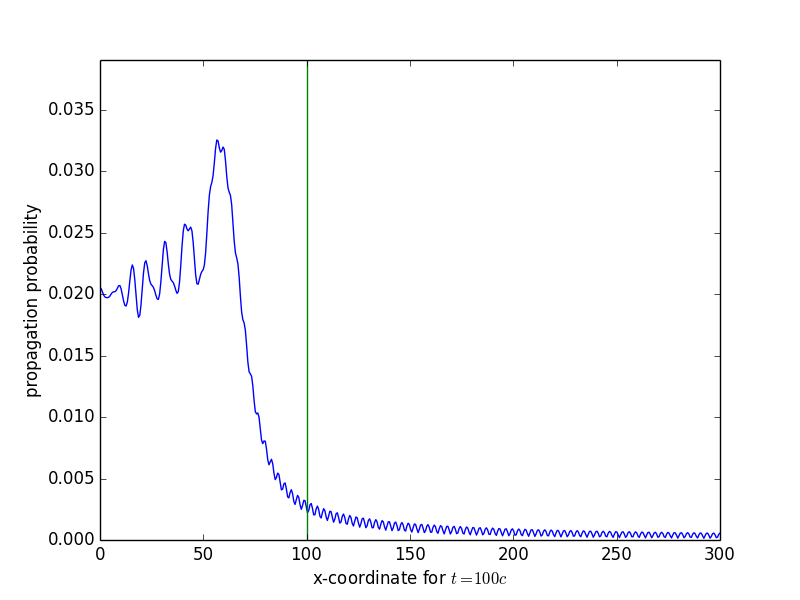
\includegraphics[width=0.6\textwidth]{free_relativistic_particle.png}
    \caption{Propagation amplitude for a free relativistic particle}
    \label{fig:free_relativistic_particle_probability}
\end{figure}

\clearpage

\begin{code}
    \captionof{listing}{Numerical integration of the relativistic free particle propagation amplitude}
    \label{code:free_relativistic_particle_amplitude}
    \begin{minted}{Python}
from numpy import sqrt, cos, sin, linspace
import scipy.integrate as integrate
import matplotlib.pyplot as plt

hbar, c, m = 1, 1, 1
TIME = 100

def function(x, t):
    def real(p):
        k = - 1 / hbar * c * (sqrt(p ** 2 + (m * c)**2)) * t
        l = 1 / hbar * p * x
        return cos(k) * cos(l) - sin(k) * sin(l)

    def imaginary(p):
        k = - 1 / hbar * c * (sqrt(p ** 2 + (m * c)**2)) * t
        l = 1 / hbar * p * x
        return sin(k) * cos(l) + cos(k) * sin(l)

    return real, imaginary

x_list = linspace(0, 3 * TIME, 500)
y_list = []

for x in x_list:
    real, imaginary = function(x, TIME)

    r = integrate.quad(real, -c, c)
    i = integrate.quad(imaginary, -c, c)
    y_list.append(sqrt(r[0] ** 2 + i[0] ** 2) / 2)

plt.xlabel("x-coordinate for $ct = {}$".format(TIME))
plt.ylabel("propagation probability")
plt.plot(x_list, y_list)
plt.plot([TIME, TIME], [0, max(y_list) * 1.2])
plt.gca().set_ylim([0, max(y_list) * 1.2])
plt.show()
    \end{minted}
\end{code}

\clearpage

In the graph \ref{fig:free_relativistic_particle_probability} we also plotted the vertical line which marks the point from which 
the event is not considered causal by our definition and the probability density should be zero there. Althought the value
in the graph is reaching the zero very quickly it is very small but non-zero in the region outside of the lightcone (i.e. on the 
right side of the vertical marking line). So we encouter the same problem as in the calculation with the non-relativistic
particle. The difference is that now we deal with an unremovable problem. We used the relativistic energy and still the theory
allowed the particle to travel faster then the speed of light with non-zero probability!
